%%%%%%%%%%%%%%%%%%%%%%%%%%%%%%%%%%%%%%%%%%%%%%%%%%%%%%%%%%%%%%%%%%%%%%%%%%%%%%%%
%2345678901234567890123456789012345678901234567890123456789012345678901234567890
%        1         2         3         4         5         6         7         8
% DOCUMENT CLASS
\documentclass[oneside,12pt]{Classes/RoboticsLaTeX}

% USEFUL PACKAGES
% Commonly-used packages are included by default.
% Refer to section "Book - Useful packages" in the class file "Classes/RoboticsLaTeX.cls" for the complete list.
\usepackage{amsmath}
\usepackage{amsfonts}
\usepackage{algorithm}
\usepackage{algorithmic}
\usepackage{multirow}
\usepackage{colortbl}
\usepackage{color}
\usepackage[table]{xcolor}
\usepackage{epigraph}
\usepackage{graphicx}
%\usepackage{subfigure}
\usepackage{caption}
\usepackage{subcaption}
\usepackage{hyperref}
\usepackage{tabularx}
\usepackage{float}
\usepackage{longtable}
\usepackage[pdftex]{graphicx}
\usepackage{pdfpages}
%\usepackage{tabularx}
\usepackage{pdflscape}
\usepackage[acronym,toc]{glossaries}
\usepackage{setspace}
\setstretch{1.5}
%\onehalfspacing
% SPECIAL COMMANDS
% correct bad hyphenation
\hyphenation{op-tical net-works semi-conduc-tor}
\hyphenation{par-ti-cu-lar mo-du-le ge-stu-re}
% INTERLINEA 1.5
%\renewcommand{\baselinestretch}{1.5}

%% ignore slightly overfull and underfull boxes
%\hbadness=10000
%\hfuzz=50pt
% declare commonly used operators
\DeclareMathOperator*{\argmax}{argmax}

% HEADER
\title{\Large{Analysis and evaluation of audio-similarity algorithms for cover and live song identification}}

\ifpdf
  \author{Martin Angelov}
  \collegeordept{MSci Computer Science with Industrial Year, Student ID 1422087}
  \university{School of Computer Science, University of Birmingham}
  \crest{
\includegraphics[width=50mm]{UoB.png}}
\else
  \author{Martin Angelov}
  \collegeordept{MSci Computer Science with Industrial Year, Student ID 1422087}
  \university{School of Computer Science, University of Birmingham}
  \crest{
\includegraphics[width=50mm]{UoB.png}}
\fi
\supervisor{Prof. Achim Jung}

% DECLARATION
% Use the following command to change the declaration text:
\renewcommand{\submittedtext}{}
\degree{}
\degreedate{}

%%%%%%%%%%%%%%%%%%%%%%%%%%%%%%%%%%%%%%%%%%%%%%%%%%%%%%%%%%%%%%%%%%%%%%%%%%%%%%%%
\makeglossaries
\loadglsentries{glossary}

\begin{document}

% A page with the abstract and running title and author etc may be
% required to be handed in separately. If this is not so, comment
% the following 3 lines:
% \begin{abstractseparate}
%   %%%%%%%%%%%%%%%%%%%%%%%%%%%%%%%%%%%%%%%%%%%%%%%%%%%%%%%%%%%%%%%%%%%%%%%%%%%%%%%%
%2345678901234567890123456789012345678901234567890123456789012345678901234567890
%        1         2         3         4         5         6         7         8
% THESIS ABSTRACT

% Use the following style if the abstract is long:
%\begin{abstractslong}
%\end{abstractslong}

\begin{abstracts}

The abstract goes here. The abstract should be self-contained and:
\begin{itemize}
    \item clearly state the problem dealt with by the thesis; \item give a synthetic description of the proposed solution;
    \item  highlight the sense in which the proposed solution enhances the state of the art.
\end{itemize}

\end{abstracts}

% \end{abstractseparate}
\begin{spacing}{1}
\maketitle
\end{spacing}

% add an empty page after title page
% \newpage\null\thispagestyle{empty}\newpage

% set the number of sectioning levels that get number and appear in the contents
\setcounter{secnumdepth}{3}
\setcounter{tocdepth}{3}


\frontmatter
%%%%%%%%%%%%%%%%%%%%%%%%%%%%%%%%%%%%%%%%%%%%%%%%%%%%%%%%%%%%%%%%%%%%%%%%%%%%%%%%
%2345678901234567890123456789012345678901234567890123456789012345678901234567890
%        1         2         3         4         5         6         7         8
% THESIS ACKNOWLEDGEMENTS

% Use the following style if the acknowledgements are long:
%\begin{acknowledgementslong}
%\end{acknowledgmentslong}

\begin{acknowledgements}


%“I don't know half of you half as well as I should like; and I like less than half of you half as well as you deserve.”
 %J.R.R. Tolkien, The Fellowship of the Ring 

Write here your acknowledgements...


\end{acknowledgements}

% %%%%%%%%%%%%%%%%%%%%%%%%%%%%%%%%%%%%%%%%%%%%%%%%%%%%%%%%%%%%%%%%%%%%%%%%%%%%%%%%
%2345678901234567890123456789012345678901234567890123456789012345678901234567890
%        1         2         3         4         5         6         7         8
% THESIS DEDICATION

\begin{dedication}

% quote
Thesis dedication goes here...
\end{dedication}

% ----------------------------------------------------------------------

%%% Local Variables: 
%%% mode: latex
%%% TeX-master: "../thesis"
%%% End: 

%%%%%%%%%%%%%%%%%%%%%%%%%%%%%%%%%%%%%%%%%%%%%%%%%%%%%%%%%%%%%%%%%%%%%%%%%%%%%%%%
%2345678901234567890123456789012345678901234567890123456789012345678901234567890
%        1         2         3         4         5         6         7         8
% THESIS ABSTRACT

% Use the following style if the abstract is long:
%\begin{abstractslong}
%\end{abstractslong}

\begin{abstracts}

The abstract goes here. The abstract should be self-contained and:
\begin{itemize}
    \item clearly state the problem dealt with by the thesis; \item give a synthetic description of the proposed solution;
    \item  highlight the sense in which the proposed solution enhances the state of the art.
\end{itemize}

\end{abstracts}


\tableofcontents
\listoffigures
\listoftables
\printglossary[title=List of Acronyms,type=\acronymtype]
% \printglossary  % Print the nomenclature (WAY TOO COMPLEX FOR ME NOW!)
% \addcontentsline{toc}{chapter}{Nomenclature}

\mainmatter
%%%%%%%%%%%%%%%%%%%%%%%%%%%%%%%%%%%%%%%%%%%%%%%%%%%%%%%%%%%%%%%%%%%%%%%%%%%%%%%%
%2345678901234567890123456789012345678901234567890123456789012345678901234567890
%        1         2         3         4         5         6         7         8
% THESIS INTRODUCTION

\chapter{Introduction}
\label{chap:introduction}
\ifpdf
    \graphicspath{{Introduction/Figures/PNG/}{Introduction/Figures/PDF/}{Introduction/Figures/}}
\else
    \graphicspath{{Introduction/Figures/EPS/}{Introduction/Figures/}}
\fi

% quote

%\setlength{\epigraphwidth}{.35\textwidth}
%\epigraph{Research is formalized curiosity.}{ Zora Neale Hurston, 1942}

% examples of sections

% \section{Motivations}
% \label{motivations}
  
% \section{Context of the Study}
% \label{context}

\section{Introduction}
\label{introduction}

Music information retrieval (MIR) is an area of analysis dedicated to extracting information from music. It combines many different disciplines of science including psychology, psychoacoustics, signal processing and computer science. One of the main aims when performing MIR solving the task of song identification, i.e. matching an audio stream to a particular song \nocite{weinstein2007music}


\section{Report structure}
\label{structure}

%%%%%%%%%%%%%%%%%%%%%%%%%%%%%%%%%%%%%%%%%%%%%%%%%%%%%%%%%%%%%%%%%%%%%%%%%%%%%%%%
%2345678901234567890123456789012345678901234567890123456789012345678901234567890
%        1         2         3         4         5         6         7         8
% THESIS Chapter

\chapter{Related terminology}
\label{chap:relatedterms}
\ifpdf
    \graphicspath{{RelatedTerminology/Figures/PNG/}{RelatedTerminology/Figures/PDF/}{RelatedTerminology/Figures/}}
\else
    \graphicspath{{RelatedTerminology/Figures/EPS/}{RelatedTerminology/Figures/}}
\fi


% short summary of the chapter `` ''
\section*{Summary}

Describe here the state of the art of the research pertaining to this thesis. This part should contain all the relevant publications in the area with the corresponding citations. The cited works should be briefly described critically assessed.
%


\section{Properties of audio}
\label{sec:audioprops}
\subsection{Test subsection}
\label{sec:subsec21}

\section{Audio transformation techniques}
\label{sec:audiotransform}
% add more sections and subsection here

%%%%%%%%%%%%%%%%%%%%%%%%%%%%%%%%%%%%%%%%%%%%%%%%%%%%%%%%%%%%%%%%%%%%%%%%%%%%%%%%
%2345678901234567890123456789012345678901234567890123456789012345678901234567890
%        1         2         3         4         5         6         7         8
% THESIS CHAPTER
% \usepackage{tikz}

\chapter{Related work}
\label{chap:relatedwork}
\ifpdf
    \graphicspath{{RelatedWork/Figures/PNG/}{RelatedWork/Figures/PDF/}{RelatedTerminology/Figures/}}
\else
    \graphicspath{{RelatedWork/Figures/EPS/}{RelatedWork/Figures/}}
\fi

% short summary of the chapter
% short summary of the chapter...

% One or more chapters should be devoted to the description of the
% proposed approach...

% In particular, this chapter describes the design adopted by this research to achieve the aims and objectives stated in the Introduction.

Cover song identification has been a very active topic of research in the last
10 years. The task has spawned many solutions, so for the scope of this project
it is infeasible for each technique to be analysed in detail - from technical
implementation details to results on datasets. To fully cover the active
developments in the research area should also examine related
research which is not the direct focus of the project.

The chapter presents an analysis of the algorithms submitted in the
\textit{Cover song identification} task, part of the Music Information Retrieval
Evaluation eXchange (MIREX) conference \cite{mirex}. The format is similar to a
competition, where participating researchers submit potential solutions to a
task and each proposal is evaluated under equal conditions. The evaluation
environment is preserved throughout the MIREX editions, so results from
different years are comparable between each other.

The study of the conference was conducted before the selection of the main
audio similarity algorithms for the project and their implementation in a
benchmark. This allowed for an informed decision on what audio features are
performing best and also ensured that algorithms not included in MIREX are
picked, to potentially present a contribution to the field.

\section{Cover song identification in MIREX 2005-2018}
\label{sec:scientificpaper}

In 2006 the MIREX conference created the \textit{Cover Song Identification}
task. The datasets used for evaluation are the MIREX 2006 US Pop Music Cover
Song dataset (1000 tracks, each track is 16-bit monophonic, 22.05 kHz sampling
rate, wav format). The dataset has 30 cover songs each represented by 11
different versions for a total of 330 files. Each of the files are then
individually run as queries for the algorithms. Each algorithm then attempts to
return the other 10 versions of the same song. The only output the submitted
algorithms should return is a \textit{number of queries} $\times$ \textit{number
of candidates} distance matrix. 

Out of the 40 submissions related to the cover song task in the MIREX conference
25 were considered. 

\subsection{Results evaluation}
\label{subsec:resultseval}

In order to determine which algorithms perform best we need to look at the
results achieved each year. From them we would then be able to determine what
audio similarity techniques have worked best so far and examine them further in
depth. 

The results outlined here are based on the statistics provided by MIREX each
year for the results of the cover song identification task. Each year MIREX
publishes the total number of covers identified (TNCI), the mean number of
covers identified (MNCI), the mean of average precisions (MAP) and the mean rank
for first correctly identified cover (MRFCIC) for each algorithm.

Let us look at the best THCI results plotted over the years for the MIREX cover
song identification task:

\begin{figure}[H]
    \centering
    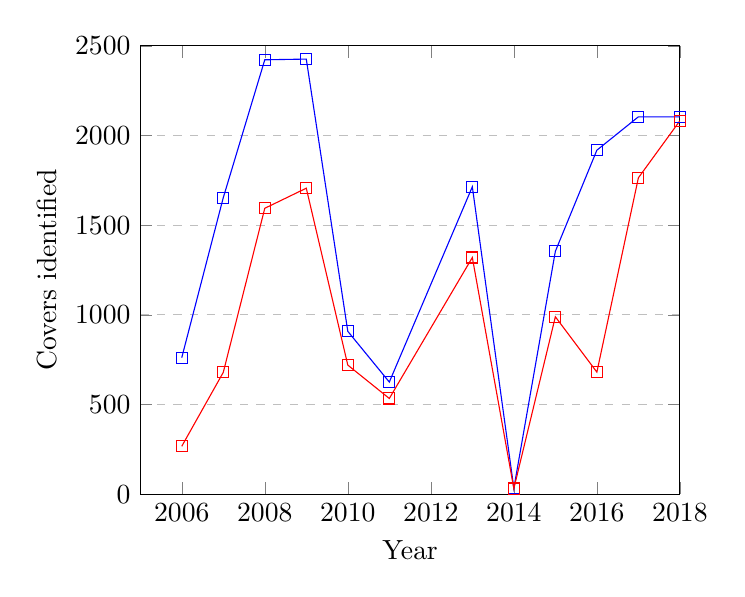
\begin{tikzpicture}
        \begin{axis}[
            /pgf/number format/.cd,
            1000 sep={},
            title={},
            xlabel={Year},
            ylabel={Covers identified},
            xmin=2005, xmax=2018,
            ymin=0, ymax=2500,
            % xtick={2006, 2008, 2010, 2012, 2014, 2016, 2018},
            xtick={},
            ytick={},
            legend pos=north west,
            ymajorgrids=true,
            grid style=dashed,
        ]
         
        \addplot[
            color=blue,
            mark=square,
            ]
            coordinates {
            (2006,761)(2007,1653)(2008,2422)(2009,2426)(2010,908)(2011,625)(2013,1714)(2014,33)(2015,1354)(2016,1918)(2017,2104)(2018,2104)
            };
            % \addlegendentry{Max THCI}
        \addplot[
            color=red,
            mark=square,
            ]
            coordinates {
            (2006,266.875)(2007,678.875)(2008,1593.875)(2009,1706)(2010,719.666666666667)(2011,533.5)(2013,1319.5)(2014,31)(2015,989)(2016,680.2)(2017,1763.75)(2018,2082)
            };
            % \addlegendentry{Average THCI}
            \end{axis}
        \end{tikzpicture}
    \caption[THCI of winning submissions in MIREX 2005-2018]{Results of the winning submissions in the period 2005-2018. The blue line represents the max THCI achieved for each year (i.e. the challenge winners). The red line outlines the average THCI for each year the task has taken place. The challenge did not run in 2005 and 2012.}
    \label{fig:mirex_results}
\end{figure}

We could see that the best performing submissions are the ones published in
2008, 2009 and 2018. 

To determine if there is a tendency into what type of audio feature is used, a
table comprising of all audio features used is compiled from the available
submissions:
\begin{figure}[H]
    \centering
    \scalebox{0.90}{
    \begin{tabular}{c|c|c}
        \textbf{Audio feature} & \textbf{Times used} & \textbf{Winner} \\
        \hline
        Chroma features & 12 & 2006, 2018 \\
        % HPCPs & 5 & 2007, 2008, 2009, 2016 \\
        % MFCCs & 2 & \\
        Harmonic Pitch Class Profiles (HPCPs) & 5 & 2007, 2008, 2009, 2016 \\
        Mel-frequency cepstral coefficients (MFCCs) & 2 & \\
        HPCP, MFCC and MFCC SSM combined & 1 & \\
        Basic Pitch Class Profiles (PCP) & 1 & \\
        Custom technique & 1 & 2014 \\
        Relationship (distance) to other songs in set & 1 & \\
        Statistical Spectrum Descriptors & 1 & \\
        Pitch line estimation & 1 & \\
    \end{tabular}
    }
    \captionof{figure}[Audio feature frequency usage in MIREX 2005-2018]{Number of times a type of audio feature is used in MIREX 2005-2018. The \textit{Winner} column indicates whether the best algorithm for the year utilises the feature.}
\end{figure}

Based on this evaluation we could see that the best audio features for measuring
song similarity are chroma features and HPCPs. Unfortunately only 7 out of the
13 winning papers were available online, so it is unclear whether they are also
using any of the features for information extraction. The \textit{custom
technique} mentioned in the table refers to an algorithm implementing a
non-conventional audio feature which achieves the worst winning result in the
MIREX competition so far  -  only  33 covers  identified (out  of  3300
possible).

Some of the main audio similarity algorithms explored in the project use chroma
features and MFCCs as audio features. Therefore in this section we only explore
the structure of HPCPs.

\subsection{Harmonic Pitch Class Profiles}
\label{subsec:hpcp}

For each pitch representing a semitone part of an equal temperament scale a
\textit{pitch class} is the set of all pitches which are all separated by an
octave from each other. Knowing that we can create a \textit{pitch class profile
(PCP)} - a vector which represents the intensities of all twelve pitch classes
\cite{fujishima1999real}. PCPs become \textit{harmonic} when they represent the
relative intensities of the pitch classes within an analysis frame in a signal
\cite{wiki:hpcp}. Straying from the general definition of a PCP they could also
be extracted over a 24 or 36-bin pitch spectrum, representing the relative
intensity of every 1/2 or 1/3 semitones respectively.

HPCPs are generally extracted using a Fourier transform to determine the
constituting frequencies in the audio stream. The resulting spectrogram is then
filtered to include only an audible spectrum of frequencies, which are then
mapped to their pitch classes. Each time frame is then normalised to obtain the
HPCP audio feature representation of a song.

\subsection{Similarity methods}
\label{subsec:simmethods}
Besides introducing the audio features which provide a song representation, a
majority of the MIREX submissions also outline the processes of measuring
similarity between songs. A set of notable similarity techniques is of interest
to background of the task. 

\textit{Dynamic time warping (DTW)} is an algorithm for measuring similarity
between two temporal sequences, which may vary in speed \cite{wiki:dtw}. The
algorithm performs a sequence alignment method, which 'bends' the sequences
non-linearly in the time dimension in order to determine the similarity
independent of other non-linear variations in the time dimension. After
sequences are aligned a rule-based matching is applied which determines the
final similarity score. Dynamic time warping has been very successful when
creating automatic speech recognition systems. The algorithm achieves great
results when used in a voice recognition system with MFCC audio features
\cite{muda2010voice}, a task not too dissimilar to cover song identification.

\paragraph{}
Because a digital audio signal is essentially a binary stream some submissions
appropriate classic information theory techniques such as \textit{Normalised
compression distance (NCD)} to establish whether two songs are covers. The
origins of NCD come from the notion of information distance, a metric that
represents the size of the shortest program required to convert one binary
object into another. We apply normalisation to the result to obtain similarity
based on the object lengths. If objects $a$ and $b$ are of length 1000000 bits
and their distance is 1000 bits, then this should be a more significant result
than having objects $c$ and $d$ of length 1000 bits with the same distance
\cite{wiki:ncd}. Given this outcome a normalised information distance (NID)
indicates that $a$ and $b$ are more similar than $c$ and $d$.

NID however is proven to not be computable or semicomputable
\cite{terwijn2011nonapproximability}. It is therefore approximated using a
compressor algorithm applied on the objects, with the NID applied to the
compressed results.
 
%%%%%%%%%%%%%%%%%%%%%%%%%%%%%%%%%%%%%%%%%%%%%%%%%%%%%%%%%%%%%%%%%%%%%%%%%%%%%%%%
%2345678901234567890123456789012345678901234567890123456789012345678901234567890
%        1         2         3         4         5         6         7         8
% THESIS CHAPTER

\chapter{The task}
\label{chap:task}
\ifpdf
    \graphicspath{{EvaluationTask/Figures/PNG/}{EvaluationTask/Figures/PDF/}{EvaluationTask/Figures/}}
\else
    \graphicspath{{EvaluationTask/Figures/EPS/}{EvaluationTask/Figures/}}
\fi


% short summary of the chapter
An evaluation task must be set based on which the algorithms are analysed,
evaluated and compared.

\section{Design} 
\label{sec:design}
The design of the evaluation task follows the general structure for an algorithm
targeted towards utilising a large-scale database. In includes taking a query
song and creating pairwise comparisons of it with any song from a song database.
The similarity score of each pair is then calculated using a cover song
identification algorithm and an ordering is created. The pair with the highest
similarity includes the database song that the algorithm has identified to be
most similar to the query song (and potentially its cover version). 

As a song database the evaluation task uses several music datasets. Each dataset
contains sets of different versions of a song. The unique identifier that
combines all versions of a single song is called a \textit{clique}. For
instance, the original version song 'Take On Me' by the Norwegian band A-ha and
its cover version created by the American punk rock artist MxPx are in the same
clique named \textit{Take On Me}. Each dataset is split into a symbolical
\textit{train} and \textit{test} sets. The train portion of the songs is
initialised as a song database, while each of the tracks in the test set is used
as a query song. During the split it is ensured that there is at least one song
from each clique in both the train and test set, so that for every query song a
cover ready to be identified is found in the song database.

The task results are produced through a benchmark written using Python
\cite{python} and storing the song database into a MongoDB \cite{mongodb}
instance. Figure \ref{fig:bencharch} shows a high-level architecture diagram of
the benchmark, which could help understand the general design of the evaluation task.

\begin{figure}[H]
    \centering
    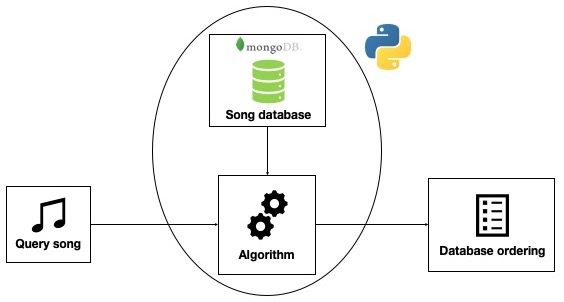
\includegraphics[width=0.75\textwidth]{EvaluationTask/benchmark_architecture.jpg}
    \captionof{figure}[Benchmark architecture diagram]{Benchmark architecture diagram}
    \label{fig:bencharch}
\end{figure}

\section{Evaluation methods and metrics} 
\label{sec:evalmethods}
All algorithms are evaluated using metrics adapted from the MIREX \textit{Cover
Song Identification} competition format. The benchmark implements the following
measurements:
\begin{itemize}
    \item \textit{mean rank (MR)} of the position of a true cover (a song from
    the same clique as the query song) in the database ordering produced by an
    algorithm
    \item \textit{mean reciprocal rank (MRR)} of the position of a true cover in
   the database ordering produced by an algorithm
   \item covers identified in the \textit{Top-K} positions of the database
   orderings for all songs, where $K$ is a number 
   \item covers identified in the \textit{Top-P} percentile of the database
   orderings for all songs, where $P$ is a number 
\end{itemize}

\section{Datasets used for evaluation} 
\label{sec:datasets}
One of the main challenges in the project was the lack of appropriate datasets,
therefore some of the datasets are self-curated using my personal music
collection. The algorithms were evaluated using the following datasets:
\begin{itemize}
    \item \textit{covers80} - a widely used by MIR researchers consisting of 80
    cliques and 164 songs \cite{covers80}. Contains original compositions and
    cover versions of them.
    \item \textit{live\_dataset} - a self-curated dataset consisting of 70
    cliques and 145 songs. Contains original compositions and professionally
    recorded, mixed and mastered live performances of them.
    \item \textit{yt\_dataset} - a self-curated dataset consisting of 16 cliques
    and 32 songs. Contains original compositions and live performances of them
    recorded from an audience perspective using a smartphone.
\end{itemize}

\textit{TODO: Mention if the songs in a dataset is included in the appendix}
%%%%%%%%%%%%%%%%%%%%%%%%%%%%%%%%%%%%%%%%%%%%%%%%%%%%%%%%%%%%%%%%%%%%%%%%%%%%%%%%
%2345678901234567890123456789012345678901234567890123456789012345678901234567890
%        1         2         3         4         5         6         7         8
% THESIS CHAPTER

\chapter{The algorithms}
\label{chap:algorithms}
\ifpdf
    \graphicspath{{Algorithms/Figures/PNG/}{EvaluationTask/Figures/PDF/}{Algorithms/Figures/}}
\else
    \graphicspath{{Algorithms/Figures/EPS/}{EvaluationTask/Figures/}}
\fi


% short summary of the chapter
The main algorithms analysed in the project are attempted to be as different as
possible from each other. This allows covering as many audio features and
similarity measuring techniques as possible. My motivations of the choice of
algorithms were influenced by the study on MIREX submissions, as well as the
overall scope of features they encompass. 

Julien Osmalsky coins the term \textit{rejector} to define a pairwise comparison
function that given two audio tracks it returns a score ranking of similarity
between both tracks \cite{osmalsky2015combining}. This term was adopted by the
project to refer to each of the algorithms examined. The relation between an
algorithm paper and its rejector term is outlined in section \ref{sec:algolist}.

The final selection includes 5 individual algorithms and an algorithm
aggregating results from 4 of them. Each of the algorithms is examined
individually, with the results from some of them combined through the rank
aggregation algorithm.


\section{Algorithms list}
\label{sec:algolist}
The analysis if performed on the following algorithm:
\begin{itemize}
    \item \textbf{Weak rejector} - Osmalskyj, Julien, Marc Van Droogenbroeck,
    and Jean-Jacques Embrechts. \textit{Enhancing cover song identification with
    hierarchical rank aggregation} \cite{osmalsky2016enhancing}
    \item \textbf{Cross-correlation rejector} - Ellis, Daniel PW, Courtenay V.
    Cotton, and Michael I. Mandel. \textit{Cross-correlation of beat-synchronous
    representations for music similarity} \cite{ellis2008cross}
    \item \textbf{Quantisation rejector} - Osmalskyj, Julien, et al.
    \textit{Combining features for cover song identification} \cite{osmalsky2015combining}
    \item \textbf{Timbre rejector} - Tralie, Christopher J., and Paul Bendich.
    \textit{Cover song identification with timbral shape sequences} \cite{tralie2015cover}
    \item \textbf{Aggregated rank rejector} - Osmalskyj, Julien, Marc Van
    Droogenbroeck, and Jean-Jacques Embrechts. \textit{Enhancing cover song
    identification with hierarchical rank aggregation}
    \cite{osmalsky2016enhancing} 
    \item \textbf{Fingerprint rejector} - Rafii, Zafar, Bob Coover, and Jinyu
    Han. \textit{An audio fingerprinting system for live version identification
    using image processing techniques} \cite{rafii2014audio}
\end{itemize}

\begin{figure}[H]
    \centering
    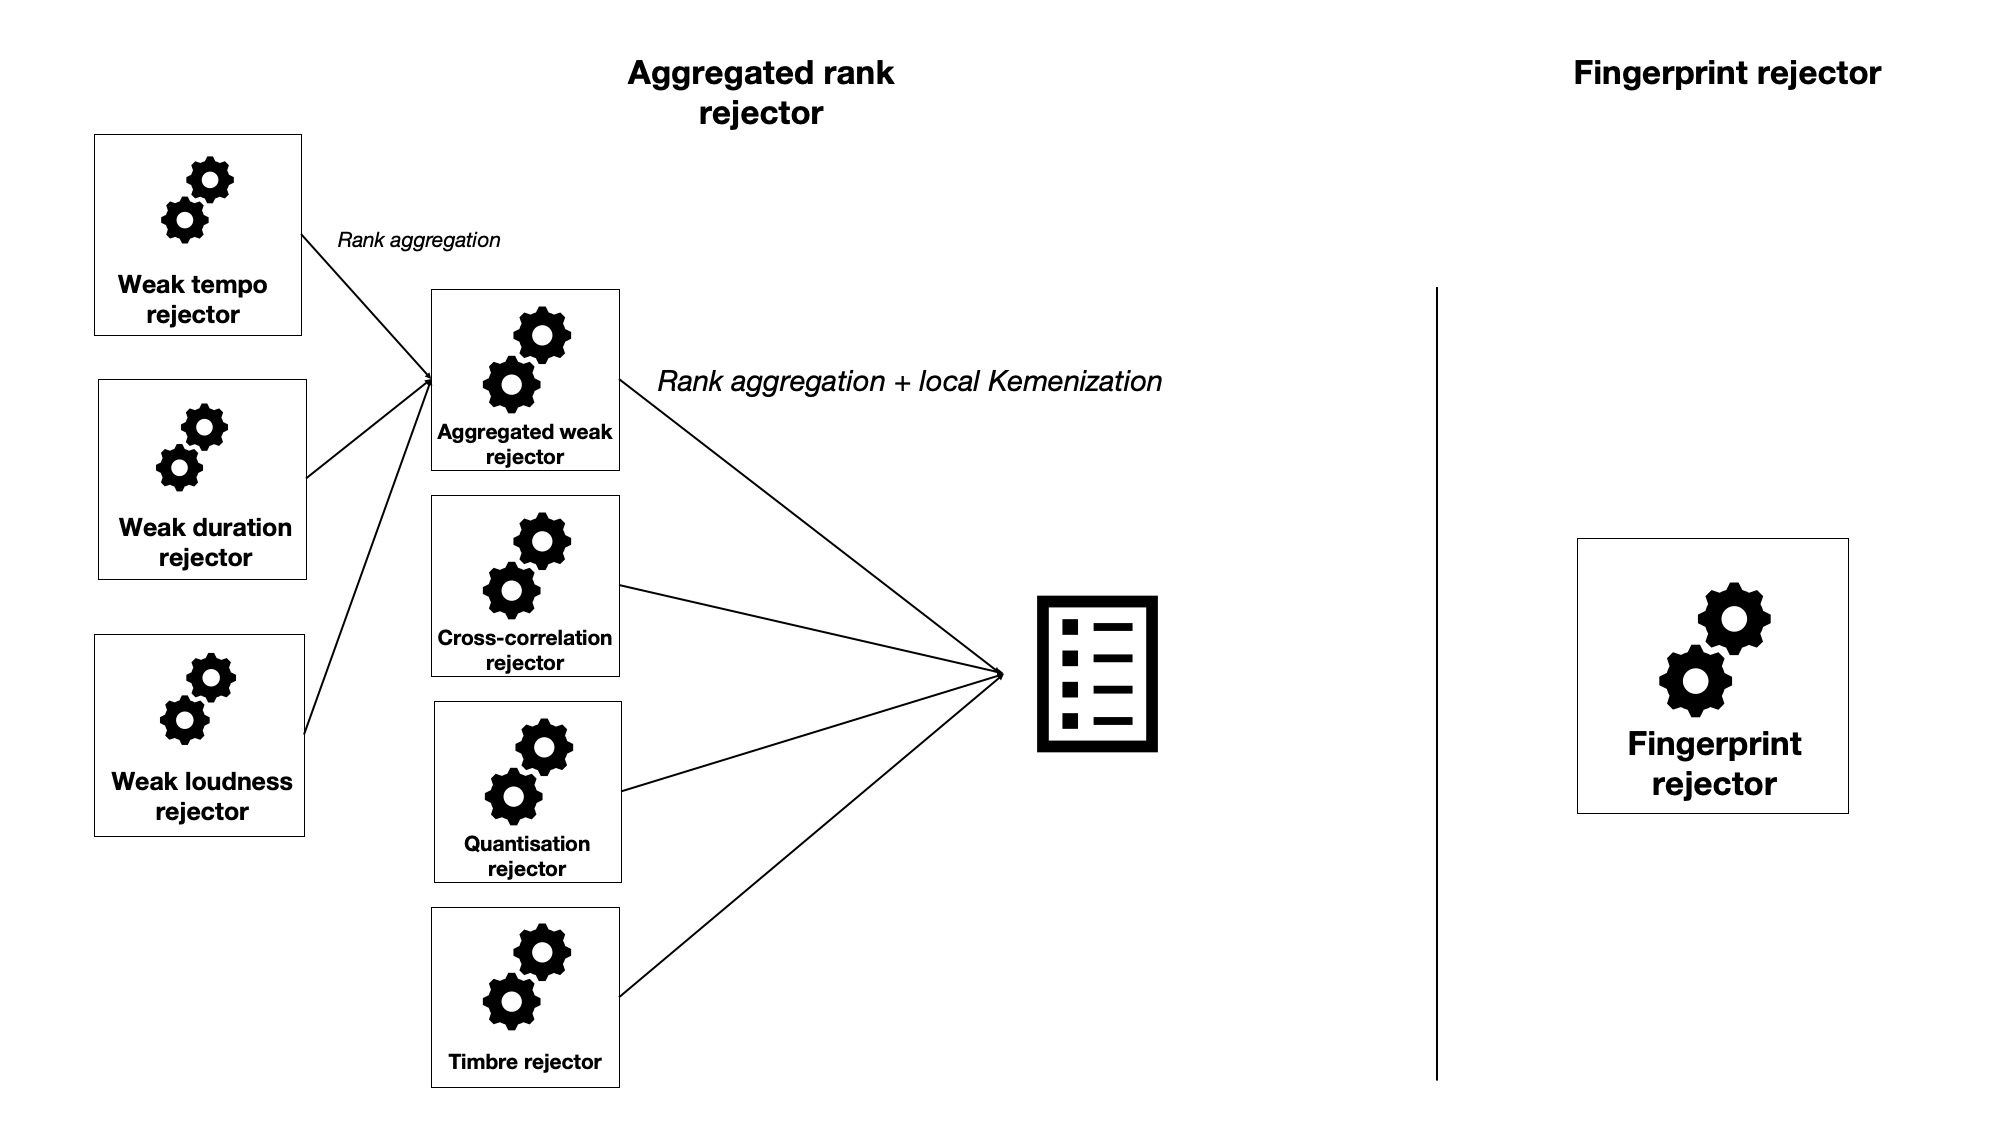
\includegraphics[width=\textwidth]{Algorithms/algorithm_diagram_3.jpg}
    \captionof{figure}[Algorithms diagram]{Diagram of chosen algorithms and the relationships between them. The aggregated rank rejector combines the results of 3 types of weak rejectors, as well as the quantisation, cross-correlation and timbre rejectors.}
    \label{fig:algorithms}
\end{figure}

\section{Weak rejector} 
\label{sec:osmalskyj}

The weak rejector takes its name from the fact that it uses global single-valued
features of sound to calculate a similarity score. Weak features include tempo,
duration, loudness, average number of beats, etc. Those audio properties are
considered 'weak' since by themselves they cannot uniquely describe a song - the
majority of pop tracks from a certain era are composed with the same tempo, for
example \cite{slowpop}. As a consequence the results from weak rejectors are
inherently insignificant are usually not considered individually, but as
part of an aggregation with other results.

Each weak rejector takes a single audio feature as song representation. The
algorithm extracts the feature from each song in a dataset and from them it
creates a training set by combining each pair of songs in different ways. For
songs $A$ and $B$ with weak feature values of $f1$ and $f2$ respectively the
minimum ($min(f1, f2)$), maximum ($max(f1, f2)$), sum ($f1 + f2$), quotient
($\frac{f1}{f2}$) and absolute value of quotient of the difference divided by
the sum ($abs(\frac{f1 - f2}{f1 + f2})$) are taken. The generated data is used
as attributes to train an ExtraTrees classifier model. Extra randomised trees or
ExtraTrees classification is a form of random forest classification. In
contrast to the regular random forest implementation, ExtraTrees uses the whole
training data for each decision tree. Rather than calculating an optimal
cut-point, it also uses a random one. The direct benefits of using this
variation of random trees are higher computational efficiency while achieving
similar perfomance on average, in addition to better results on some specific
problems \cite{geurts2006extremely}.

The evaluation datasets used in this project are too small to generate an
ExtraTrees model which performs even adequate classification of songs. To gather
sufficient training data the weak features of 12,104 songs are extracted from
the music streaming service Spotify \cite{spotify}. The tracks are chosen based
on clique groupings from the SecondHandSongs (SHS) \cite{shs} dataset - the
largest dataset of covers songs aimed at academic research. While the full
dataset is difficult to obtain, information about the cliques structure within
it is easy to find. The extracted data is then combined into pairs using the
procedure outlined in the previous paragraph. A binary class is then assigned to
each pair entry depending on whether the pair of songs are covers or not.
Afterwards the training data is further split into a training set of 3773
cliques (8653 songs) and validation set containing 1573 cliques (3451 songs).
The metric used to validate the model performance is the area under the receiver
operating characteristic (ROC) curve - a curve resulting from the plot of the
true positive against the false positive rate of the validation results. ROC
analysis of such form is suitable as a validation metric for the selection of an
optimal model because it is independent of any potential cost function or cost
distribution \cite{wiki:roc}. Because we are solely working with weak feature
information the we can only validate based on correct and incorrect produced results.

After the training phase is complete each of the evaluation datasets is
converted into the training set format and passed to the model for class
prediction. The output result is a probability of every pair of songs being
covers. Grouping the results per song produces a database ordering that is
required by the evaluation task.

\section{Cross-correlation rejector} 
\label{sec:weakfeatures}
The cross-correlation rejector uses chroma features as the main audio feature
describing each song. Chroma is another name for pitch class profiles, i.e. the
intensity distribution in each of the twelve pitch classes part of the chromatic
scale \cite{fujishima1999real}. Any feature that at its core uses chroma to
represent a song is a chroma feature. That is why the terms harmonic pitch class
profiles (HPCP) and chroma features have a very similar definition, in fact
HPCP is a type of chroma feature. The main difference between chroma features is
their method of extraction. Using chroma features produces a chromagram - a
pitch class versus time plot showing the intensity of each pitch class at any
time point (Figure \ref{fig:chromagram}).

\begin{figure}[H]
    \centering
    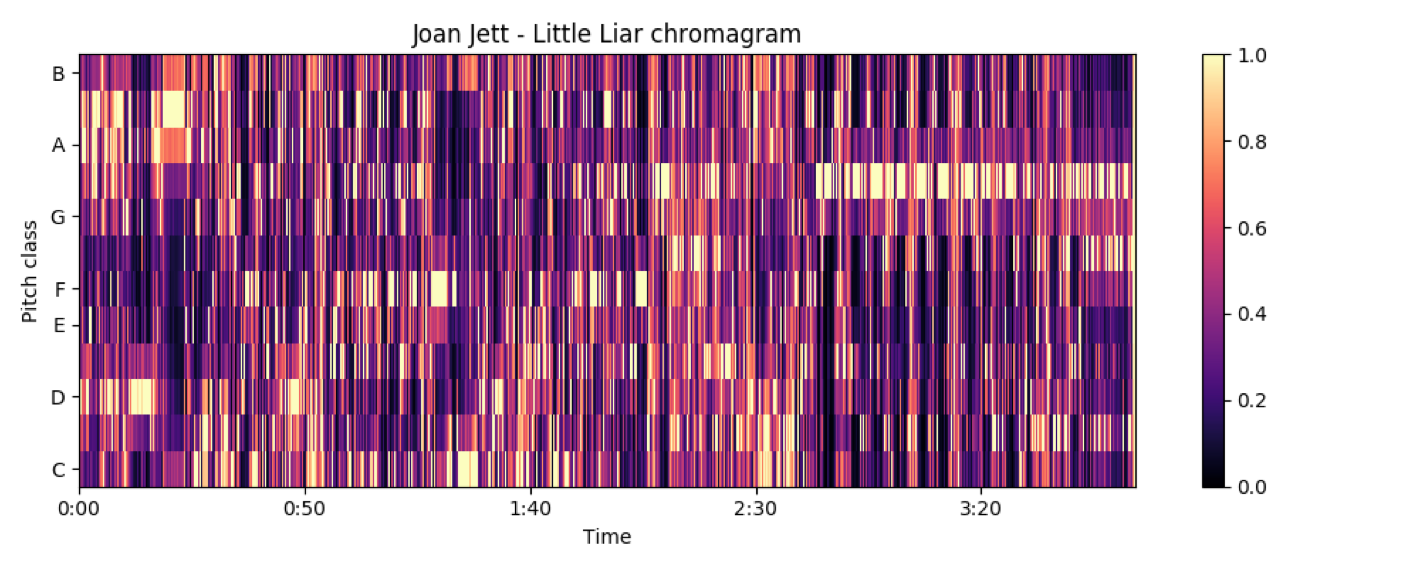
\includegraphics[width=\textwidth]{Algorithms/chromagram_picture.png}
    \captionof{figure}[Chromagram]{Chromagram of the song \textit{Little Liar} by Joan Jett}
    \label{fig:chromagram}
\end{figure}

The chroma features in the cross-correlation rejector are extracted using
short-time Fourier transform (STFT). This is an audio transformation which
performs Fourier transform on short segments of a signal and aims to determine
the local frequency and phase changes over the small signal intervals.
\textit{FINISH THIS}

\section{Quantisation rejector}
\label{sec:ccs}
\section{Timbre rejector} 
\label{sec:quantisation}
\section{Aggregated rank rejector} 
\label{sec:timbre}
\section{Fingerprint rejector} 
\label{sec:rankaggregation}


%%%%%%%%%%%%%%%%%%%%%%%%%%%%%%%%%%%%%%%%%%%%%%%%%%%%%%%%%%%%%%%%%%%%%%%%%%%%%%%%
%2345678901234567890123456789012345678901234567890123456789012345678901234567890
%        1         2         3         4         5         6         7         8
% THESIS CHAPTER

\chapter{Evaluation benchmark}
\label{chap:benchmark}
\ifpdf
    \graphicspath{{Algorithms/Figures/PNG/}{EvaluationTask/Figures/PDF/}{Algorithms/Figures/}}
\else
    \graphicspath{{Algorithms/Figures/EPS/}{EvaluationTask/Figures/}}
\fi


% short summary of the chapter

The benchmark implementing the algorithm was targeted for solely personal use,
therefore the majority of its functionality is not easily accessible through a
form of a user interface. The output that most functions generate is verbose and
is intended to assist with the analysis of the inner workings of an algorithm.
Overall it is recommended the benchmark to be used as a software library, rather
than a standalone tool.

Following on the design of the evaluation task any usage of the benchmark
requires a MongoDB instance to store audio features and act as a song
database on figure \ref{fig:bencharch}. A Docker Compose recipe is available in
the \textit{misc/docker} directory of the project GitLab repository for quick
spawning a MongoDB container.

\section{Implementation details} 
\label{sec:implementation}

As mentioned before the whole benchmark is implemented in Python 3.7. To perform
audio feature extraction from a song the benchmark utilises Librosa, a library
for  audio and music processing \cite{librosa}. Librosa offers various functions
to extract all required audio features using different Fourier transforms, as
well as the ability to separate a song into beat frames. The software was also
written by the authors of the cross-correlation rejector \cite{ellis2008cross},
and its beat tracker implementation is the core of beat tracking for the timbre
rejector implementation \cite{tralie2015cover}. Because of that Librosa was
the preferred choice for audio analysis library over other options \cite{aubio}
\cite{pyAudioAnalysis}.

Connections between the benchmark and the database are accommodated
through the official MongoDB Python package called \textit{PyMongo}
\cite{pymongo}. The audio feature extraction functionality in the benchmark
could potentially serve as a middleware between Librosa and PyMongo in future
MIR-related projects.

Other general matrix operations are achieved using \textit{NumPy}, a popular
scientific computation Python package \cite{numpy}.

The benchmark is mainly targeted to be run on sets of query songs, rather than
individual songs. Each algorithm implementation however has a
\textit{run\_on\_test\_set} and \textit{run\_on\_query\_song} functions, which
initiate an algorithm runs on a set of query songs or an individual query track.

\section{Algorithm implementations in the benchmark} 
\label{sec:algostructure}
This section offers documentation on the exact parameters used during each
algorithm implementation. It complements all information from chapter
\ref{chap:algorithms}. 
\subsection{Weak rejectors}
\label{subsec:weakrejectorimplementation}
Tempo, loudness and duration weak rejectors have been produced by the benchmark.
Each rejector is in the form of a classifier model, with an implementation for
ExtraTrees classification provided by the \textit{scikit-learn} Python library
\cite{scikit-learn}. The trained models are stored into the database, so that
they can be reused to produce classifications during an algorithm execution. The
maximum depth for each tree in the model is set to 20. Due to memory concerns
the classifier is trained using batches of data rather than on the full training
set at the same time. A tree is added for each training phase using a batch of
data. For batches of approximately 42,000 pairs the overall number of trees in
the trained model is 1819. The low maximum depth of a tree combined with the
number of trees helps reduce model overfitting \cite{osmalsky2016enhancing}.

The ROC scores returned by the trained models used in the results generation are
$0.5$ for the duration and tempo classifiers and $0.53$ for the loudness
classifier.

\subsection{Cross-correlation rejector}
\label{subsec:ccsimplementation}

Chroma features for the cross-correlation rejector are extracted using STFT with
a window size of 2048 samples and a hop length of 512 samples. The extraction of
the beat frames of a song is done using an initial tempo estimate of 240 beats
per minute (bpm), a value mentioned in the original algorithm implementation.
The cross-correlation of two chromagrams is performed on row pairings using the
NumPy \textit{correlate} function. The resulting cross-correlation matrix is
normalised by the size of the smaller chromagram so that the maximum possible
peak value is 1.

\subsection{Quantisation rejector}
\label{subsec:quantisationimplementation}

The process of extracting chroma vectors in the quantisation rejector is
completely identical to the cross-correlation rejector implementation. The
trained K-means model forms 200 cluster centers and uses \textit{k-means++}
(initial random selection of first cluster center with every following center
selected using a weighted probability based on distance to all previously chosen
centers) as an initialisation model. The K-Means clustering implementation was
provided by scikit-learn. The training phase involved approximately 42,000
chroma vectors extracted from the train sets of the datasets. The finalised
model is again stored into the database for persistence.

The achieved inertia of the best performing K-means model was 5633.

\subsection{Timbre rejector}
\label{subsec:timbreimplementation}

The extraction of MFCCs for the timbre rejector was achieved through the
\textit{mfcc} function provided by Librosa, which inherently uses a discrete
cosine transform (DCT), a Fourier-related transform similar to DFT. The window
size of the transform is dependent on the tempo of a song and is determined by
the function $\frac{60}{tempo} * sr$, where $sr$ is the sample rate of the song.

The beat tracking takes 3 initial guesses for tempo (60, 100, 180) and 3
dimensions (100 $\times$ 100, 200 $\times$ 200, 300 $\times$ 300) are examined
for size of the self-similarity matrix for each track. This leads to the
construction of 9 self-similarity matrices (SSMs) for each database or query song.

An implementation of the Smith-Waterman algorithm provided by the creator of the
algorithm is directly used to generate similarity scores.

The current version of the timbre rejector runs considerably slower compared to
the other audio similarity algorithms. While a run of the rest of the algorithms
usually takes a relatively short time (up to 30 minutes per dataset) the
timbre-based algorithm takes a variable time between 2 and 6 hours to return a
result for a single query song of the dataset. A potential reason for the long
run time could be the high computational costs associated with handling 9 SSM
representations for a single database song. Each SSM represented as a NumPy
matrix takes a lot of storage space - the total size of the SSMs for all
database songs for the \textit{covers80} dataset takes almost 90 GB in MongoDB.
Retrieving such a significant amount of data from the database for every query
song, combined with the construction of a cross-similarity matrix for each SSM
results in a very slow task. Even utilising lazy loading, a pre-processing step
required due to all SSM results from the database being too big to fit in
memory, does not result in any noticeable improvement of the time for execution.


% Make sure to mention and make a discussion on why the timbre rejector runs slow

\subsection{Rank aggregation rejector}
\label{subsec:rankaggrimplementation}
The rank aggregation rejector takes advantage of the \textit{min, max, median}
and \textit{mean} functions in NumPy to determine an aggregated rank from an
array of ranks.

\subsection{Fingerprint rejector}
\label{subsec:fingerprintimplmentation}

As per algorithm specification, the constant Q transform (CQT) applied on query
segments and database songs uses a window size of 512 samples, a range of 120
frequency channels and a minimum frequency of 130.81 Hz (equivalent to the C3
note). The conversion of the resulting spectrogram to a binary image is
performed using a adaptive thresholding implementation provided by the
\text{scikit-image}, a Python image processing library. The neighbourhood sizes
considered are 15 and 35. Hamming similarity is calculated using the
\textit{hamming} function from \textit{SciPy}, another scientific calculation
package. 

\section{Benchmark result format} 
\label{sec:resformat}

The result of an algorithm run on a query song is stored as an entry in a
MongoDB collection. Apart from the actual similarity scores each entry also
includes metadata allowing for easy understanding of the results:

\begin{figure}[H]
   \centering 
   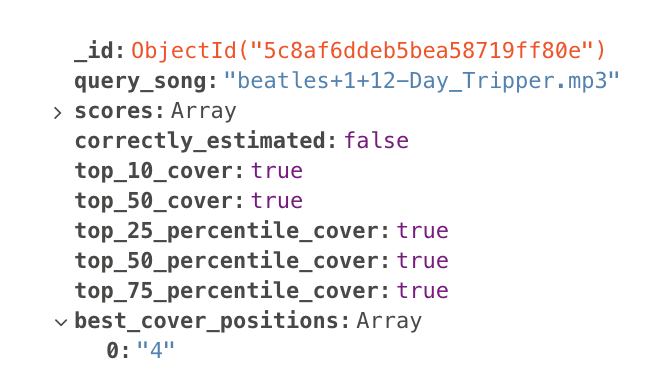
\includegraphics[width=0.5\textwidth]{Benchmark/overallresult.png}
   \captionof{figure}[Example of an algorithm result in database]{An example of an algorithm result for a single query song. The representation accommodates for a quick retrieval of the \textit{Top-K} and \textit{Text-P} evaluation metrics}
   \label{fig:overallresult}
\end{figure}

The verbose similarity scores are available in the \textit{scores} array:

\begin{figure}[H]
    \centering
    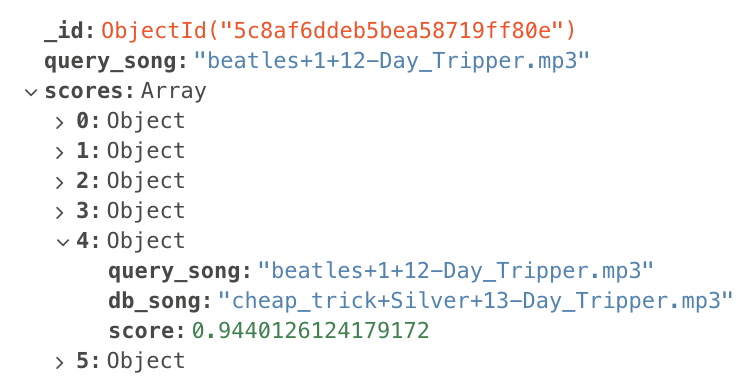
\includegraphics[width=0.5\textwidth]{Benchmark/scoresresult.png}
    \captionof{figure}[Example of verbose similarity score in database]{Verbose scores stored in the database}
    \label{fig:scoresresult}
\end{figure}

The benchmark supports exporting the evaluation metrics defined in chapter
\ref{chap:task} as CSV files.
%%%%%%%%%%%%%%%%%%%%%%%%%%%%%%%%%%%%%%%%%%%%%%%%%%%%%%%%%%%%%%%%%%%%%%%%%%%%%%%%
%2345678901234567890123456789012345678901234567890123456789012345678901234567890
%        1         2         3         4         5         6         7         8
% THESIS CHAPTER

\chapter{Results and experimentation}
\label{chap:results}
\ifpdf
    \graphicspath{{Algorithms/Figures/PNG/}{EvaluationTask/Figures/PDF/}{Algorithms/Figures/}}
\else
    \graphicspath{{Algorithms/Figures/EPS/}{EvaluationTask/Figures/}}
\fi


% short summary of the chapter
\section*{Summary}
Details all the results of your study here ( exploits graphics for results visualisation). 
This chapter should also contain a full discussion, interpretation and evaluation of the results. 



\section{Best results} 
\label{sec:bestres}
\section{Comparison to results from papers} 
\label{sec:rescomparison}
\section{Result analysis} 
\label{sec:resanalysis}


%%%%%%%%%%%%%%%%%%%%%%%%%%%%%%%%%%%%%%%%%%%%%%%%%%%%%%%%%%%%%%%%%%%%%%%%%%%%%%%%
%2345678901234567890123456789012345678901234567890123456789012345678901234567890
%        1         2         3         4         5         6         7         8
% THESIS CHAPTER

\chapter{Further work}
\label{chap:furtherwork}
\ifpdf
    \graphicspath{{Algorithms/Figures/PNG/}{EvaluationTask/Figures/PDF/}{Algorithms/Figures/}}
\else
    \graphicspath{{Algorithms/Figures/EPS/}{EvaluationTask/Figures/}}
\fi


% short summary of the chapter
% \section*{Summary}
Details all the results of your study here ( exploits graphics for results visualisation). 
This chapter should also contain a full discussion, interpretation and evaluation of the results. 



% \section{Lack of datasets} 
% \label{sec:gv2}
% \section{Lack of universal comparison metric?} 
% \label{sec:gv2}
% \section{Academic papers algorithm description} 
% \label{sec:gv2}


%%%%%%%%%%%%%%%%%%%%%%%%%%%%%%%%%%%%%%%%%%%%%%%%%%%%%%%%%%%%%%%%%%%%%%%%%%%%%%%%
%2345678901234567890123456789012345678901234567890123456789012345678901234567890
%        1         2         3         4         5         6         7         8
% THESIS CHAPTER

\chapter{Challenges}
\label{chap:challenges}
\ifpdf
    \graphicspath{{Algorithms/Figures/PNG/}{EvaluationTask/Figures/PDF/}{Algorithms/Figures/}}
\else
    \graphicspath{{Algorithms/Figures/EPS/}{EvaluationTask/Figures/}}
\fi


% short summary of the chapter
\section*{Summary}
Details all the results of your study here ( exploits graphics for results visualisation). 
This chapter should also contain a full discussion, interpretation and evaluation of the results. 



\section{Lack of datasets} 
\label{sec:lackdatasets}
\section{Lack of universal comparison metric?} 
\label{sec:lackmetric}
\section{Academic papers algorithm description} 
\label{sec:lackalgopapers}


%%%%%%%%%%%%%%%%%%%%%%%%%%%%%%%%%%%%%%%%%%%%%%%%%%%%%%%%%%%%%%%%%%%%%%%%%%%%%%%%
%2345678901234567890123456789012345678901234567890123456789012345678901234567890
%        1         2         3         4         5         6         7         8
% THESIS CHAPTER

\chapter{Project management}
\label{chap:management}
\ifpdf
    \graphicspath{{Algorithms/Figures/PNG/}{EvaluationTask/Figures/PDF/}{Algorithms/Figures/}}
\else
    \graphicspath{{Algorithms/Figures/EPS/}{EvaluationTask/Figures/}}
\fi


% short summary of the chapter
\section*{Summary}
Details all the results of your study here ( exploits graphics for results visualisation). 
This chapter should also contain a full discussion, interpretation and evaluation of the results. 



\section{Using GitLab} 
\label{sec:gitlab}
\section{Canvas logs} 
\label{sec:canvaslogs}
\section{other? Gantt chart?} 
\label{sec:ganttchart}


%%%%%%%%%%%%%%%%%%%%%%%%%%%%%%%%%%%%%%%%%%%%%%%%%%%%%%%%%%%%%%%%%%%%%%%%%%%%%%%%
%2345678901234567890123456789012345678901234567890123456789012345678901234567890
%        1         2         3         4         5         6         7         8
% THESIS CONCLUSIONS
\def\baselinestretch{1}
\chapter{Conclusions}
\label{chap:conclusions}
\ifpdf
    \graphicspath{{Conclusions/Figures/PNG/}{Conclusions/Figures/PDF/}{Conclusions/Figures/}}
\else
    \graphicspath{{Conclusions/Figures/EPS/}{Conclusions/Figures/}}
\fi
\def\baselinestretch{1.0}

% quote

Conclusions should summarize the problem, the solution and its main innovative features, outlining future work on the topic or application scenarios of the proposed solution.



\appendix
%%%%%%%%%%%%%%%%%%%%%%%%%%%%%%%%%%%%%%%%%%%%%%%%%%%%%%%%%%%%%%%%%%%%%%%%%%%%%%%%%
%2345678901234567890123456789012345678901234567890123456789012345678901234567890
%        1         2         3         4         5         6         7         8
% THESIS APPENDIX

\chapter{Gesture Vocabulary} 
\label{chap:appendixA}


\begin{figure}
    \centering
    \includegraphics[width=0.8\textwidth]{Chapter4/Figures/Figures/gv.PNG}
    \caption{Proposed gesture vocabulary}
    \label{fig:gs}
\end{figure}


%\chapter{Survey}
\label{chap:appendixB}


%\begin{figure}
%\setboolean{@twoside}{false}
% Uncomment the follow line to show the survey
\includepdf[pages=1-,scale=0.8,pagecommand={}]{Appendix2/gbhri3_format.pdf}
%\end{figure}

%\begin{figure}
 %\centering 
 %\includegraphics{Appendix2/gbhri3_format.pdf}
%\end{figure}
%\bibliographystyle{Classes/RoboticsBiblio}    % bibliography style
\bibliographystyle{ieeetr}
\renewcommand{\bibname}{References}           % change default name Bibliography to References
\bibliography{References/references}          % References file
\addcontentsline{toc}{chapter}{References}    % add References to contents page

%\addcontentsline{toc}{section}{References}
\nocite{*}
\end{document}
